\begin{abstract}
Applications of computer-vision in agriculture have significant
potential for improving the precision and efficiency of several
in-field operations, including spraying and cultivation.
Systems which utilize imaging for hydraulic
control, such as for inter-row cultivation, can be used to obtain
additional state information which may be used to positively affect the system's
performance. Of primary interest is estimating the
motion of vehicle-mounted orthographic cameras in order to obtain
ground-speed and orientation feedback. We propose a feature-based
method for real-time motion estimation of agricultural vehicles and
implements via image analysis without the need for RTK GPS. The SURF,
SIFT, and ORB feature-descriptor algorithms were evaluated for their
suitability on varying surfaces for speeds up 18 km/h. Keypoint
matching was conducted using knn-matching with cross-checking and the
computer-vision estimation was compared against RTK
GPS. Possible applications are discussed, including a model for
orientation compensation of pivoting-hitch cultivator steering systems.
\end{abstract}

\section{Introduction}
\lipsum[1]

\section{Literature Review}
Emerging applications for computer-vision on agricultural implements
Row-crop cultivation
Strip tillage
Post-harvest spraying
Motion feedback is very useful for such applications
Orientation
Responsiveness
Incorporating speed detection into these systems can be problematic
RTK GPS can be expensive
Low-cost GPS units are less reliable
Fifth-wheels can suffer from slippage

\section{Methodology}

% --- BEGIN Camera Model --- %
\subsection{Camera Model}
An outdoor (dust-tight, water-tight) CMOS camera with 640x480 pixel
resolution was mounted to the front of a New Holland T5050 (New
Holland Agriculture, Turin, Italy) tractor in-line with a crop row to
obtain a video stream of the plants passing beneath the equipment. The
camera lens had an aperture of 2.4, a 6 mm focal point, and a 4:3
aspect ratio, which translated to a 43$^{\circ}$ horizontal field of view and
32.9$^{\circ}$ vertical field of view. For the specifications, the camera
provided approximately 1.15 mm/px resolution when mounted 1.0 m above
the ground and oriented orthogonally to the testing surface. In order
to maximize the overlap between consecutive images at higher travel
speeds, the camera was oriented width-wise in the direction of
travel. The camera sensor was capable of automatically adjusting
white-balance for varying lighting conditions and could capture images
at a rate of approximately 25 frames per second. Additionally, the
CMOS sensor of the camera was not IR-filtered and the camera enclosure
was equipped with 24 infrared LEDs. This allowed the device to be used
effectively in a wide range of ambient lighting conditions and was
rated to a minimum illumination of 0.5 Lux.

In order to determine the ground speed of the vehicle using
computer-vision, an application was developed with the Python OpenCV
platform using the SURF (Speeded Up Robust Features) keypoint matching
algorithm \cite{bay}. The application was developed to run on an
Intel i7 powered VMC3501-K (Nexcomm, Taiwan). A Trimble AgGPS RTK
receiver position directly above the camera was used to obtain
geographic longitude and latitude, time, and GNSS signal quality for
each data point produced by the computer-vision algorithm. To account
for variance in the subject depth, the distance from the camera to the
surface, an ultrasonic sensor with 1 cm accuracy was mounted at the
same vertical height as the camera.

\begin{figure}
  \centering
  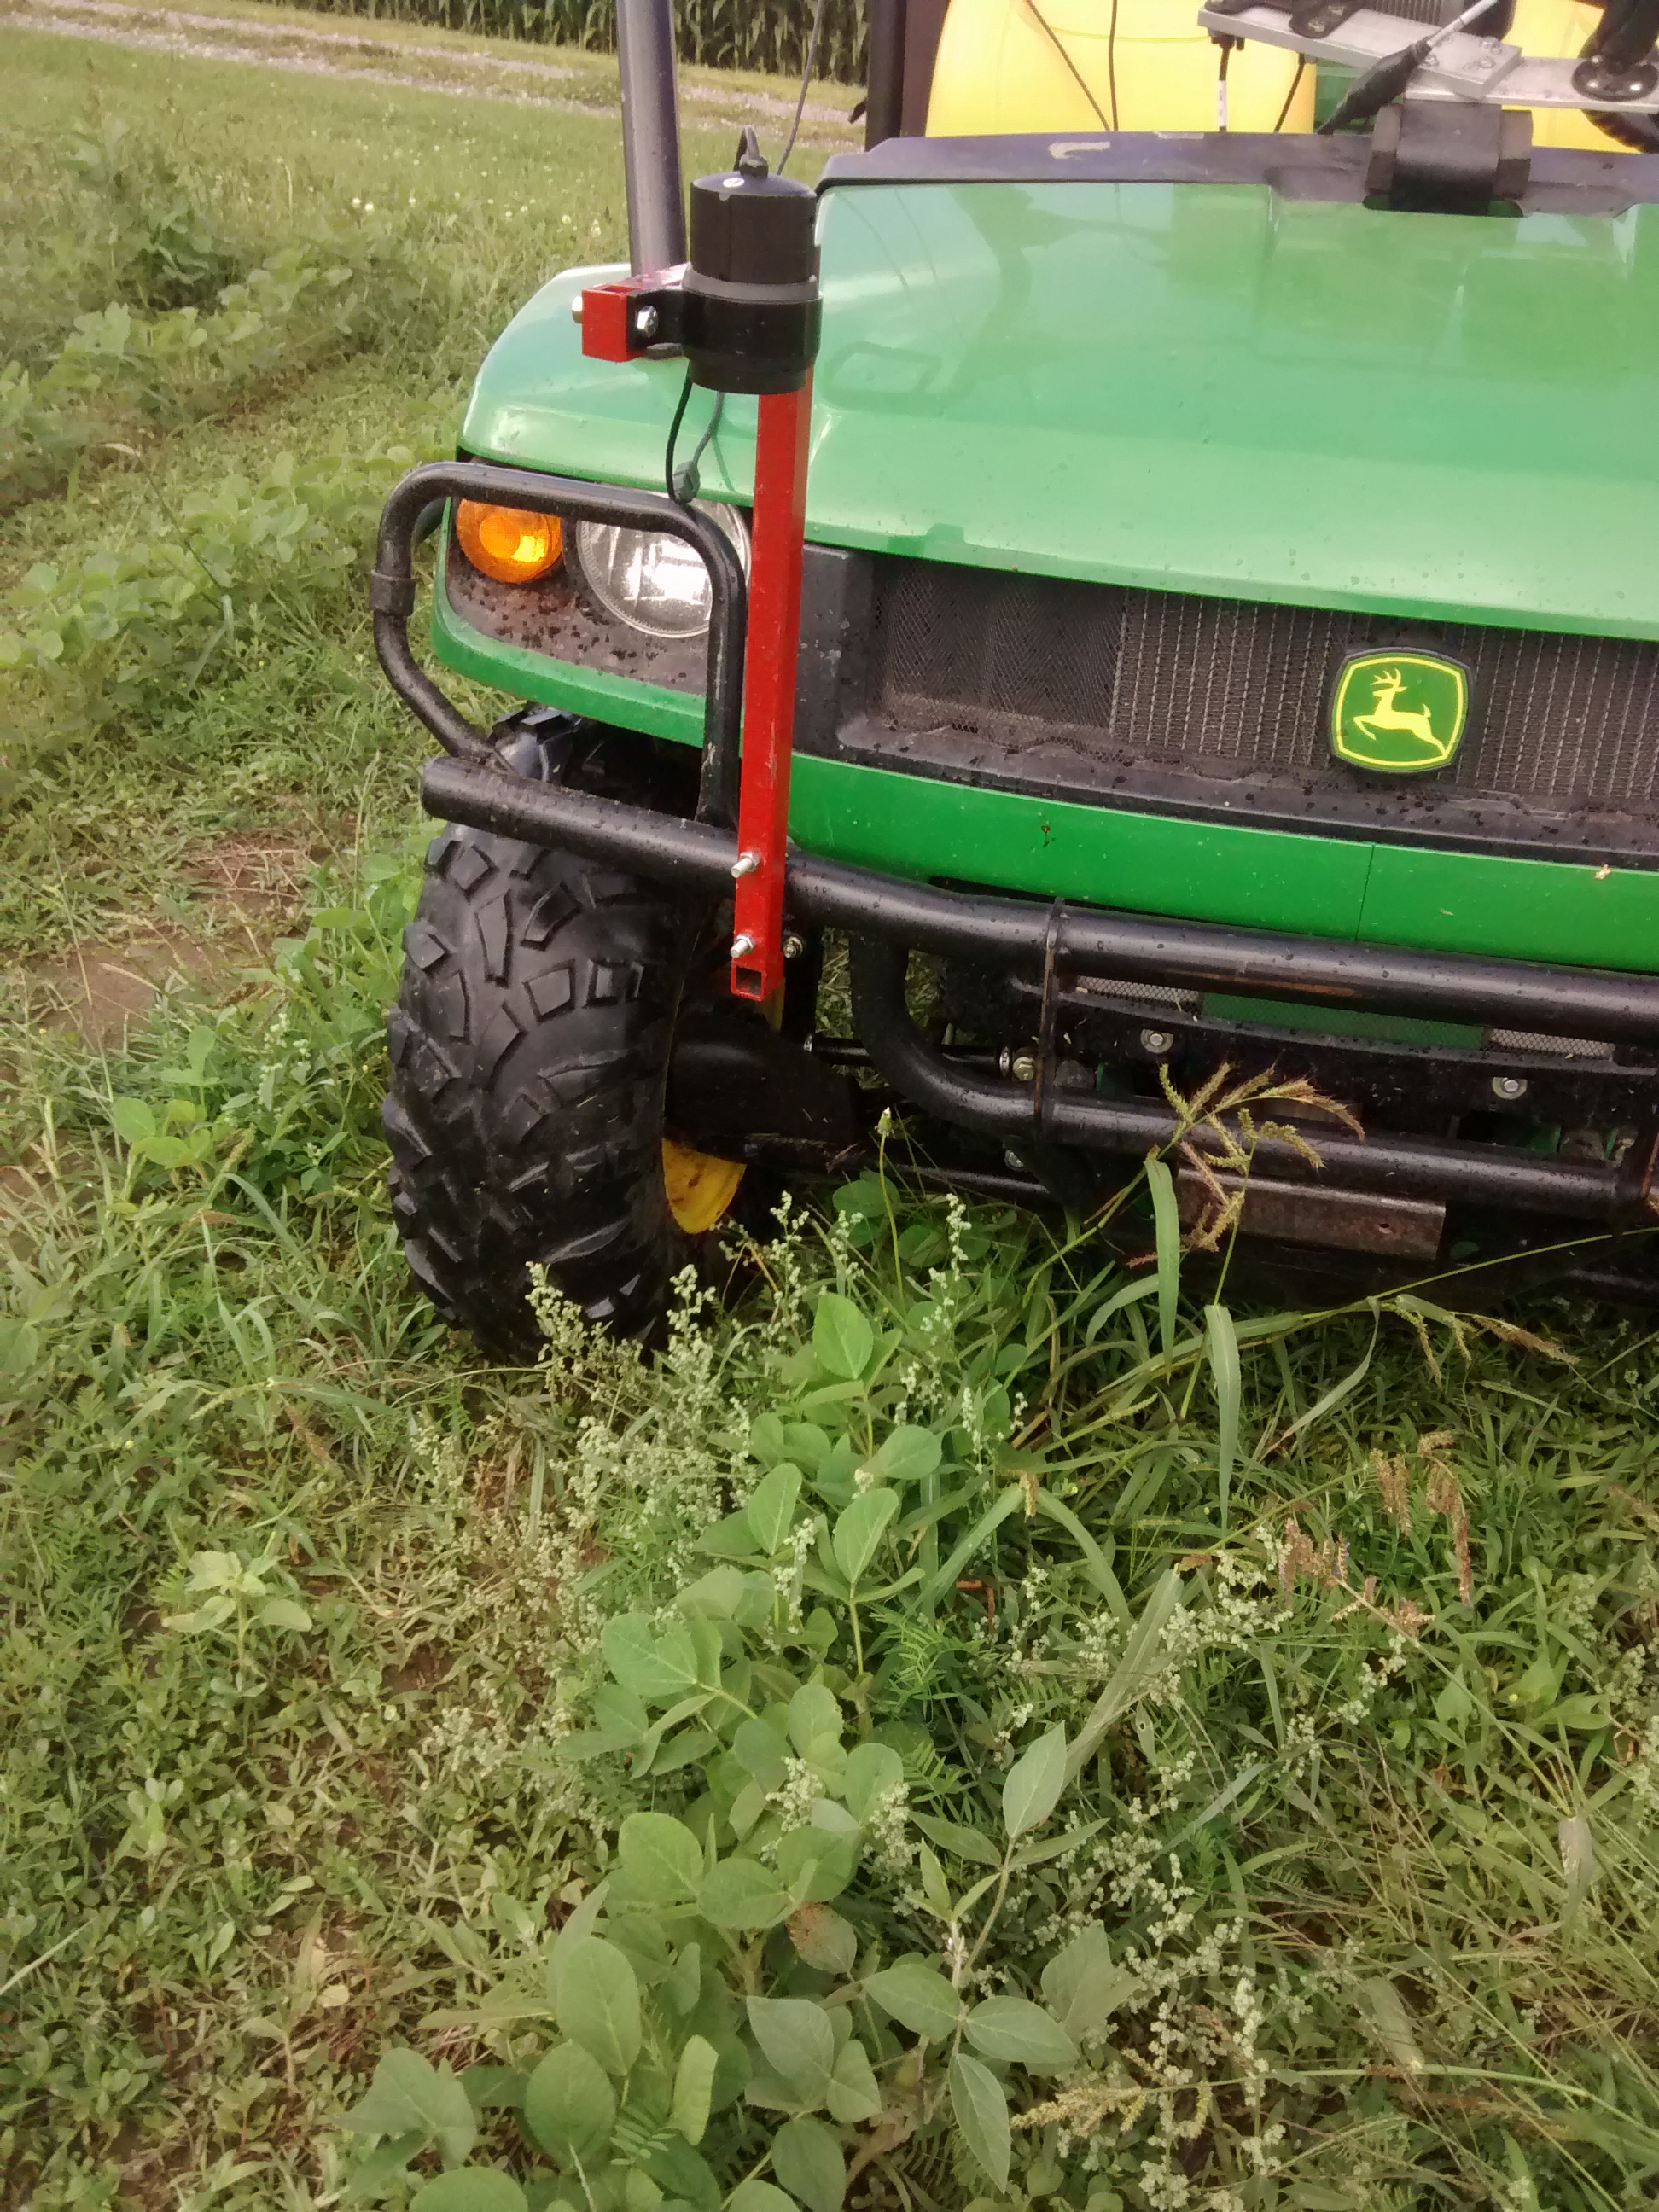
\includegraphics[width=0.8\textwidth,natwidth=610,natheight=642]{camera_bracket.jpg}
  \caption{Camera Bracket}
  \label{fig:camera_bracket}
\end{figure}

Using the checkboard pattern, the lens and projection distortion was corrected.
\begin{figure}
  \centering
  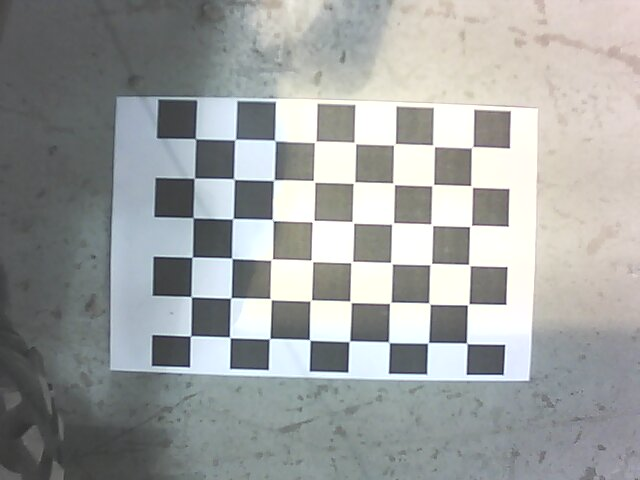
\includegraphics[width=0.8\textwidth,natwidth=610,natheight=642]{calibration.jpg}
  \caption{Checkerboard camera calibration}
  \label{fig:calibration}
\end{figure}
% --- END Camera Model --- %

% --- BEGIN Image Processing --- %
\subsection{Image Processing}
To determine the ground speed of the tractor using computer vision,
the proposed algorithm captures two consecutive RGB images from the
camera, M1 and M2, at times t1 and t2, respectively. Each image matrix
is then transformed to grayscale by the following formula:

Contrast-limited adaptive histogram equalization (CLAHE) was used to
optimize the gray-scale images. If any histogram bin exceeds the
specified contrast limit of 40, those pixels are clipped and
distributed uniformly to other bins before applying histogram
equalization. After equalization, to remove artifacts in tile borders,
bilinear interpolation is applied.
% --- END Image Processing --- %

% --- BEGIN Keypoint Matching --- %
\subsection{Keypoint Matching}
Both sets of descriptors, D1 and D2, are then matched using k-Nearest
Neighbors brute-force matching, where each of the keypoint descriptors
of M1 are compared to those of M2. For the regression, two best
matches were found for each query descriptor. This process results in
a set consisting of pairs of possible keypoint matches and the
corresponding error terms:

To filter the array of possible matches for good matches, for each
pair of possible matches the error of each match is compared to the
other. If the match has a first error term (eA) which is less than
half of the second error term (eB), then the point is considered a
good match and is stored to set Q.  

\begin{figure}
  \centering
  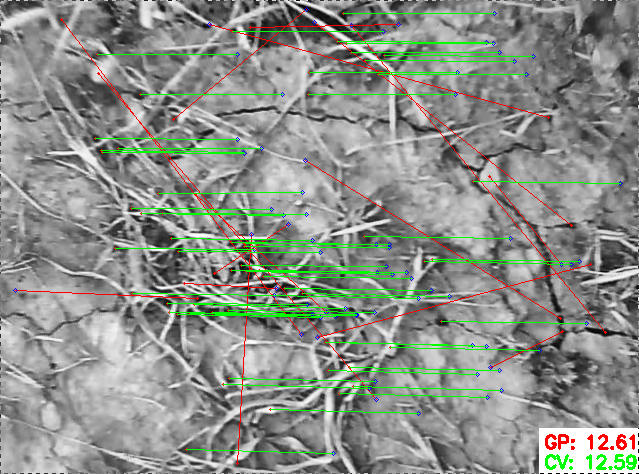
\includegraphics[width=0.8\textwidth,natwidth=610,natheight=642]{keypoint_tracking.png}
  \caption{Keypoint tracking.}
  \label{fig:keypoint_tracking}
\end{figure}

The true position of keypoints identified by the algorithm is
determined by the perspective of the imaging device. 

\begin{equation}
\centering
\lambda = \frac{W}{2.0 * tan(\frac{\alpha}{2})}
\label{eq:geometric}
\end{equation}
\begin{flushleft}
Where f is the focal length, W is the width of the image, $\alpha$ is
the field of view, K is the zoom-factor, S is the subject depth  (1000
mm), $\rho$ is the pitch
(0.0 radians).
\end{flushleft}

For each pair of matched keypoints $M_{1}$ and $M_{2}$,
i.e. $(x_{1},y_{1})$ and $(x_{2},y_{2})$, their coordinates are
projected from pixel-space to real-space with the following
transformation to correct for lens and perspective distortion.

\begin{equation}
r = sqrt(x^2 + y^2)
\label{eq:hypothenus}
\end{equation}

\begin{equation}
\binom{X}{Y} = K \times \binom{x}{y}
\begin{pmatrix}
  c_{1} & c_{1} & \cdots & c_{n}
\end{pmatrix}
\begin{pmatrix}
  1 \\
  r^2 \\
  \vdots \\
  r^{2n}
\end{pmatrix}
\label{eq:undistort}
\end{equation}
\begin{flushleft}
where $c_{i}$ are the transform coefficients deteremined by calibration.
\end{flushleft}

The velocity of each keypoint between the two consecutive images was
calculated by taking the change in distance between the coordinates in $M_{1}$ and
$M_{2}$ divided by the rate of image capture (f):
\begin{equation}
  \text{atan2}(y,x) = 
  \begin{cases}
    \text{arctan}(\frac{y}{x})  & \quad \text{if } x \ge 0  \\
    \text{arctan}(\frac{y}{x}) + \pi  & \quad \text{if } x \le 0
    \text{ and } y \ge 0 \\
    \text{arctan}(\frac{y}{x}) - \pi  & \quad \text{if } x \le 0
    \text{ and } y < 0  \\
    +\frac{\pi}{2}  & \quad \text{if } x = 0
    \text{ and } y > 0  \\
    -\frac{\pi}{2}  & \quad \text{if } x = 0
    \text{ and } y < 0 \\
    \text{undefined}  & \quad \text{if } x = 0
    \text{ and } y = 0  \\
  \end{cases}
\label{eq:atan2}
\end{equation}

\begin{equation}
\binom{v}{\theta} = \binom{\frac{\sqrt((X_{2} - X_{1})^2 + (Y_{2} - Y_{1})^2)}{f}}{\text{arctan2}(X_{2} - X_{1}, Y_{2} - Y_{1})}
\label{eq:pts2vector}
\end{equation}
\begin{flushleft}
Where v is the velocity, and $\theta$ is the direction, relative to
the cameras orientation along the horizontal centerline.
\end{flushleft}

The set of vectors was filtered by clustering by histogram and
selecting for dominant vector angle within a tolerance of 0.05
radians. Consistently removes stationary objects and false pairs
without being computationally intensive. Additionally, since the
dominant vector angle is used, despite its simplicity this approach is
orientation-agnostic.
% --- END Keypoint Matching --- %

% --- BEGIN Trials --- %
\subsection{Field Trials}
To ensure precise estimation of speed, the following procedures were conducted prior to testing:
Ensure orientation of camera within 1 degree.
Ensure pitch of camera within 1 degree
Ensure height of camera at 1000 mm to concrete surface
Six (6) surface types
Pavement
Gravel
Soil / Residue
Turf Grass
Hay Grass
Mature Soy
For each surface type, five (5) videos were collected
0 km/h to 18 km/h to 0 km/h in ~45 seconds
% --- END Trials --- %

% --- BEGIN Results --- %
\section{Results}

\begin{table}[h]
  \centering
  \caption{RMSE and 95$^{th}$ Percentile
    with respect to crop-stage.} 
  \scalebox{0.6}{
    \begin{tabular}{lcccccccc}
      \toprule
      \multirow{2}[10]{*} & \multicolumn{7}{c}{RMSE (cm)} \\
      \cmidrule(1r){2-8}
      & 0-3 & 3-6 km/h & 6-9 km/h & 6-12 & 12-15 &
      15-18 km/h & \bf total \\
      \midrule
      pavement & 21.33 $\pm$ 6.78 & 20.92 $\pm$ 7.97 & 66.33 $\pm$ 16.07
      & 66.15 $\pm$ 16.71 & 38.39 $\pm$ 0.81 & 38.35 $\pm$ 0.79 &
      133.34 $\pm$ 18.60  \\ 
      gravel & 0.50 $\pm$ 6.43 & 19.36 $\pm$ 8.11 & 63.69 $\pm$ 15.01
      & 65.67 $\pm$ 16.49 & 38.86 $\pm$ 0.23 & 38.9 $\pm$ 0.29 &
      145.55 $\pm$ 15.61 \\ 
      grass & 21.33 $\pm$ 6.78 & 20.92 $\pm$ 7.97 & 66.33 $\pm$ 16.07
      & 66.15 $\pm$ 16.71 & 38.39 $\pm$ 0.81 & 38.35 $\pm$ 0.79 &
      133.34 $\pm$ 18.60  \\
      hay & 21.33 $\pm$ 6.78 & 20.92 $\pm$ 7.97 & 66.33 $\pm$ 16.07
      & 66.15 $\pm$ 16.71 & 38.39 $\pm$ 0.81 & 38.35 $\pm$ 0.79 &
      133.34 $\pm$ 18.60 \\ 
      soy & 21.33 $\pm$ 6.78 & 20.92 $\pm$ 7.97 & 66.33 $\pm$ 16.07
      & 66.15 $\pm$ 16.71 & 38.39 $\pm$ 0.81 & 38.35 $\pm$ 0.79 &
      133.34 $\pm$ 18.60 \\ 
      soil & 21.33 $\pm$ 6.78 & 20.92 $\pm$ 7.97 & 66.33 $\pm$ 16.07
      & 66.15 $\pm$ 16.71 & 38.39 $\pm$ 0.81 & 38.35 $\pm$ 0.79 &
      133.34 $\pm$ 18.60 \\ 
      corn residue & 21.33 $\pm$ 6.78 & 20.92 $\pm$ 7.97 & 66.33 $\pm$ 16.07
      & 66.15 $\pm$ 16.71 & 38.39 $\pm$ 0.81 & 38.35 $\pm$ 0.79 &
      133.34 $\pm$ 18.60 \\ 
      \bottomrule  
    \end{tabular}}
  \label{table:travel_speed}
\end{table}

% --- END Results --- %

\section{Discussion}
\lipsum[1]

\subsection{Applications}

\lipsum[1]

\section{Conclusion}
\lipsum[1]